\begin{equation}
    - \Sigma^{\text{Fock}}_{\vb*{k} \sigma \omega} = \begin{gathered}
        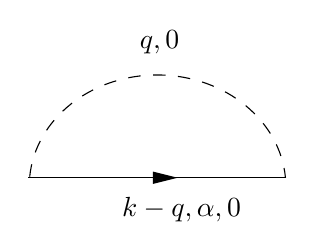
\begin{tikzpicture}[x=0.75pt,y=0.75pt,yscale=-1,xscale=1]
            %uncomment if require: \path (0,300); %set diagram left start at 0, and has height of 300
            
            %Straight Lines [id:da2955007220043213] 
            \draw    (152,181) -- (275.71,181) ;
            %Shape: Arc [id:dp18804672248212917] 
            \draw  [draw opacity=0][dash pattern={on 4.5pt off 4.5pt}] (152.72,180.56) .. controls (155.45,152.87) and (182.29,131.3) .. (214.8,131.6) .. controls (247.11,131.89) and (273.43,153.68) .. (275.93,181.17) -- (214.31,185.34) -- cycle ; \draw  [dash pattern={on 4.5pt off 4.5pt}] (152.72,180.56) .. controls (155.45,152.87) and (182.29,131.3) .. (214.8,131.6) .. controls (247.11,131.89) and (273.43,153.68) .. (275.93,181.17) ;
            %Straight Lines [id:da9181481581871234] 
            \draw    (224,181.12) ;
            \draw [shift={(224,181.12)}, rotate = 180] [fill={rgb, 255:red, 0; green, 0; blue, 0 }  ][line width=0.08]  [draw opacity=0] (12,-3) -- (0,0) -- (12,3) -- cycle    ;
            
            % Text Node
            \draw (204.5,109.08) node [anchor=north west][inner sep=0.75pt]    {$\boldsymbol{q},0$};
            % Text Node
            \draw (196,189.08) node [anchor=north west][inner sep=0.75pt]    {$\boldsymbol{k}-\boldsymbol{q}, \alpha, 0$};
            \end{tikzpicture}                      
    \end{gathered} = \frac{1}{V} \sum_{\vb*{q}, \alpha} (- V_{\vb*{q}}) (- n^0_{\vb*{k} - \vb*{q}, \alpha} \delta_{\sigma \alpha}),
    \label{eq:lowerest-self-energy-fock-fermi-liquid}
\end{equation}